\documentclass{beamer}
\author{Vajna Mikl\'{o}s}

\setbeamertemplate{background canvas}[vertical shading][bottom=white,top=structure.fg!25]

\usetheme{Warsaw}
\setbeamertemplate{headline}{}
\setbeamertemplate{footline}[page number]
\setbeamersize{text margin left=0.5cm}
  
\usepackage[magyar, english]{babel}

\usepackage{times}
\usepackage[utf8]{inputenc}
\usepackage[T1]{fontenc}

\begin{document}

\title{Nyílt forráskódú irodai programkomponensek vállalati környezetbe való integrációjának vizsgálata és implementációja}
\date{2012. január 24.}

\frame{\titlepage}

\begin{frame}
\frametitle{Tartalomjegyzék}
\begin{enumerate}
\item Bevezető
\item Motiváció
\item Feladat leírása
\item Megoldott feladatok
\begin{enumerate}
\item Dokumenummenedzsment
\item Munkafolyamatok
\end{enumerate}
\item Tesztelés
\item Jövőbeli lehetőségek
\item Összefoglalás
\item Válaszok a bírálat kérdéseire
\end{enumerate}
\end{frame}

\begin{frame}
\frametitle{Bevezető}
\begin{itemize}
\item Szoftverfejlesztéshez bevett eszköz a verziókezelő
\item Előnyeit technikai előképzettséggel nem rendelkező felhasználók is szeretnék élvezni
\item Megoldás: dokumentummenedzsment rendszerek
\item Kliensek nyílt forráskódú migrációja $\Leftrightarrow$ nem tudnak ezekkel a rendszerekkel kommunikálni
\item Dokumentumokon végzett műveletek munkafolyamat részei
\item Probléma: manuális szinkronban tartás
\begin{itemize}
\item dokumentum és a munkafolyamat állapota
\end{itemize}
\end{itemize}
\end{frame}

\begin{frame}
\frametitle{Motiváció}
\begin{itemize}
\item Az egyik legelterjedtebb dokumentummenedzsment rendszer a Sharepoint
\item Létezik nyílt forráskódú alternatívája, pl. Alfresco
\item Ehhez létezik OpenOffice.org kiterjesztés: OPAL.
\item Írjuk át a kiterjesztést, hogy Sharepointtal tudjon kommunikálni!
\item A kiterjesztés kommunikálhatna a munkafolyamat-kiszolgálóval is egyben
\item Elérhető nyílt forráskódú REST API-t támogató munkafolyamat-motor, pl. jBPM
\end{itemize}
\begin{figure}[H]
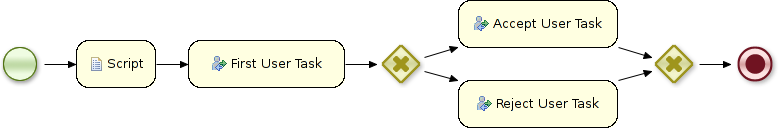
\includegraphics[width=75mm,keepaspectratio]{decision-bpmn.png}
\end{figure}
\end{frame}

\begin{frame}
\frametitle{Feladat leírása}
\begin{figure}[H]
\includegraphics[width=75mm,keepaspectratio]{test-arch-wf-hu.pdf}
\end{figure}
\begin{itemize}
\item Sharepoint funkcionalitás felmérése
\item LibreOffice kiterjesztés készítés elsajátítása
\item Létező kiterjesztés portolása LibreOffice-hoz, átírása Sharepointra
\item Alfrescohoz és Sharepointhoz lehessen egyidejűleg kapcsolódni
\item Létező jBPM funkcionalitás felmérése, igény szerint bővítése
\item jBPM integráció megvalósítása a kiterjesztésben
\end{itemize}
\end{frame}

\begin{frame}
\frametitle{Megoldott feladatok}
\framesubtitle{Dokumentummenedzsment: Sharepoint funkcionalitás felmérése}
\begin{itemize}
\item Hitelesítés: HTTP Basic, NTLM.
\item Használt protokollok: Vermeer RPC, SOAP.
\item Használati esetek gyűjtése (felhasználói felület):
\begin{itemize}
\item Munkaterületek létrehozása, törlése
\item Munkaterületeken belüli mappák létrehozása, listázása, törlése
\item Mappákban tárolt dokumentumok olvasása, írása
\item Dokumentumok verziókezelése: listázás, visszaállítás, törlés, olvasás
\item Dokumentumok kivétele, visszaadása, kivétel elvetése
\end{itemize}
\end{itemize}
\end{frame}

\begin{frame}
\frametitle{Megoldott feladatok}
\framesubtitle{Dokumentummenedzsment: Létező kiterjesztés átírása Sharepointra}
\begin{itemize}
\item Protokoll visszafejtése: Wireshark, vázlatos referencia MSDN-ről.
\item Megfigyelt rendszer: Microsoft Office 2007, Microsoft Sharepoint 2007.
\item OPAL Java kódjának átírása Sharepointhoz.
\item Különálló Sharepoint library.
\item Szerveroldali komponens telepítése nem szükséges.
\end{itemize}
\end{frame}

\begin{frame}
\frametitle{Megoldott feladatok}
\framesubtitle{Dokumentummenedzsment: Alfresco és Sharepoint egyidejűleg}
\begin{itemize}
\item Ahol szerver oldalon migráltak, ott általában Alfresco-ra.
\item Cél: ha a klienseket korábban migrálják, a szerveroldali migráció után változatlanok maradhassanak a kliensek.
\item Megoldás: VTI modul Alfresco-hoz, Sharepoint protokoll szerveroldali implementációja.
\item Problémák: hiányos implementáció.
\end{itemize}
\end{frame}

\begin{frame}
\frametitle{Megoldott feladatok}
\framesubtitle{Dokumentummenedzsment: Kiterjesztés architektúra}

\begin{figure}[H]
\includegraphics[width=100mm,keepaspectratio]{uno-java-hu.pdf}
\end{figure}
\end{frame}

\begin{frame}
\frametitle{Megoldott feladatok}
\framesubtitle{Munkafolyamat-integráció}
Tervezett funkcionalitás:
\begin{itemize}
\item Felhasználóhoz rendelt feladatokhoz tartozó dokumentumok listázása
\item Dokumentum mentése után a munkafolyamat léptetése (igény szerint)
\item Csoportfeladatok vállalása és visszaadása
\item Maszkolt dokumentum-hozzáférés: csak az aktív munkafolyamat-feladathoz tartozó szakasz szerkeszthető
\item Munkafolyamat-döntések a mentés során
\item Audit log elérése
\end{itemize}
\end{frame}

\begin{frame}
\frametitle{Megoldott feladatok}
\framesubtitle{Munkafolyamat-integráció: jBPM bővítés}
\begin{figure}[H]
\includegraphics[width=70mm,keepaspectratio]{bpm-console-hu.pdf}
\end{figure}
\begin{itemize}
\item Csak az audit log nem volt elérhető REST API-n
\item Az ehhez szükséges információ eddig is tárolásra került relációs adatbázisban
\item Szükséges módosítások: jBPM és REST kiszolgáló közötti belső API, valamint a REST kiszolgáló publikus API-ja
\item Már befejezett munkafolyamatok, csomópontok, feladatok elérése
\end{itemize}
\end{frame}

\begin{frame}
\frametitle{Tesztelési környezet}

Funkcionális tesztelés, használati esetek alapján. Környezet:
\begin{itemize}
\item Linux, Windows
\item Eclipse 3.5
\item LibreOffice 3.3 és 3.4
\item SharePoint 2007 Enterprise
\item jBpm 5.1.0.Final
\end{itemize}

\end{frame}

\begin{frame}
\frametitle{Jövőbeli lehetőségek}
\begin{itemize}
\item Jogosultságkezelés, linkek, taskok kezelése
\item CMIS: Content Management Interoperability Services
\item GUI többszálúsítása
\item Natív filepickerek használata
\item jBPM mellett más munkafolyamat-motorok támogatása
\item BPM konzolhoz audit log támogatás
\end{itemize}
\end{frame}

\begin{frame}
\frametitle{Összefoglalás}
\begin{itemize}
\item A diplomaterv eredményeként egy -- nyílt forráskódú irodai
programcsomagból használható -- egyszerű Sharepoint és jBPM kliens készült el.
\item Ennek részeként elkészült egy különállú Sharepoint Java kliens könyvtár,
mely korábban nem volt elérhető.
\item Használatához szerveroldali komponens telepítése nem szükséges.
\item Több platformon (OpenOffice, LibreOffice) fut, operációs rendszerek
közötti hordozhatóságát a Java biztosítja.
\item A dokumentumtár és a munkafolyamat-motor integrálása újdonság, más irodai
programkomponensben sem volt idáig elérhető.
\end{itemize}
\end{frame}

\begin{frame}
\frametitle{Válaszok a bírálatban szereplő kérdésekre}
\begin{itemize}
\item \textbf{Tervezi-e a továbbfejlesztést, ha igen, akkor milyen irányban?}
Karbantartás jelleggel mindenképp, viszont a jBPM módosításokat upstream-elése
prioritás
\item \textbf{Miért döntött a kiterjesztés típusú megoldás mellett?} Mivel a
másik irányban nehezebb az átjárás a kétfajta megoldás között
\item \textbf{Vannak-e tervek arra vonatkozóan, hogy a kiterjesztés része
legyen a LibreOffice és OpenOffice.org alaptelepítésnek.} Első lépésben az
Extension Repository-ba feltöltés a terv, indokolt népszerűség esetén
alaptelepítésbe való integráció javaslat

\end{itemize}
\end{frame}

\end{document}
